\chapter{Solar radiation in South Africa and load curve covering concept}\label{Solar power in South Africa}
South Africa is one of the country with the highest potential for generating solar thermal electricity in the word. Figure \ref{DHI-DIF} shows  the daily sum of global irradiation in Aberdeen, United Kingdom and Upington, South Africa. The yearly share of diffuse irradiation in Aberdeen overlaps 60 \%. In winter month the share reaches 90 \%. The share in Upington is approximately 25 \% and is in total significantly higher than Aberdeen. The direct comparison shows also the difference of the solar irradiation between northern and southern hemisphere during the year. It is obviously, that the seasons are the other way around between both hemispheres.



This chapter shows energy impact from the sun and how it is distributed in SA. Furthermore the chapter comprised the current situation of solar power plants in SA.
\begin{figure}[h!] % DHI-DFI
\centering
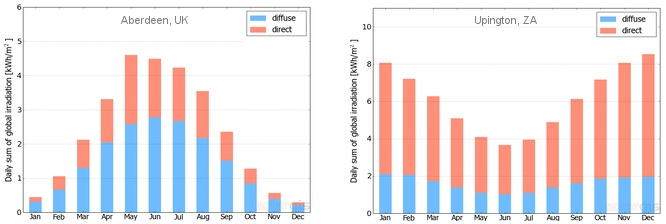
\includegraphics[width=1\linewidth]{FIG/DHI-DIF}
\caption[Long-term monthly variability of direct (DNI) and diffuse (DHI) irradiaton throughout the year for Aberdeen in the United Kingdom and Upington in South Africa.]{Long-term monthly variability of direct (DNI) and diffuse (DHI) irradiaton throughout the year for Aberdeen in the United Kingdom and Upington in South Africa \cite{SolarGIS2015}.}\label{DHI-DIF}
\end{figure} 
\section{Solar radiation}
The most important solar radiation parameters for designing a solar power plant are here defined:
\begin{itemize}
\item \textbf{GHI} (kWh/m\textsuperscript{2}/a or W/m\textsuperscript{2}): Global Horizontal Irradiance is the total amount of shortwave radiation received from above by a horizontal surface. It includes direct (beam) and a diffuse (scattered) irradiation. This value is of particular interest to PV or solar water heater with a fixed inclined angle.
\item \textbf{DNI} (kWh/m\textsuperscript{2}/a or W/m\textsuperscript{2}): Direct Normal Irradiance is the amount of solar radiation received per unit area by a surface that is always held perpendicular (or normal) to the rays that come in a straight line from the direction of the sun at its current position in the sky. Diffuse irradiation is totally excluded from the DNI. This quantity is of particular interest to  installations that track the position of the sun.
\item \textbf{DHI} (kWh/m\textsuperscript{2}/a or W/m\textsuperscript{2}): Diffuse Horizontal Irradiance is the amount of radiation received per unit area by a surface that does not arrive on a direct path from the sun, but has been scattered by molecules and particles in the atmosphere and comes equally from all directions.
\end{itemize}
Furthermore is irradiance understood as instantaneous density of solar radiation incident on a given surface, typically expressed in W/m\textsuperscript{2} and irradiation is the sum of irradiance over a time period expressed in J/m\textsuperscript{2} or more commonly used in Wh/m\textsuperscript{2}. The connection between the solar radiation parameters is shown in Equation \ref{GL_GHI}.The angle $\theta_\text{z}$ is the angle between the direction of the sun and the zenith (directly overhead).
\begin{align}
GHI=DNI*\cos(\theta_{z})+DHI \label{GL_GHI}
\end{align}
Figure\ref{irradiation} shows the solar GHI and the DNI data for the country. It is shown, that the ceiling value for GHI can be more than 2~300~kWh/m\textsuperscript{2}/a, whereas in some parts of the country the DNI  value attains about 2~900~kWh/m\textsuperscript{2}/a. This is significantly high than in the most regions worldwide, therefor SA is predestined for using solar technologies. The figure shows, that the southeastern coastline has predominantly the lowest irradiance values. The solar irradiation rise significant in the inland. The highest GHI can be find close to the Namibian boarder in the northeast of the country. The direct beam is also at highest in the western part of SA. The area around Springbok in the province Northern Cape has the highest DNI value of the country.
%% Abbildung GHI und DNI
\begin{figure}[h!]
        \centering
        \begin{subfigure}[b]{0.5\textwidth}
                \centering
                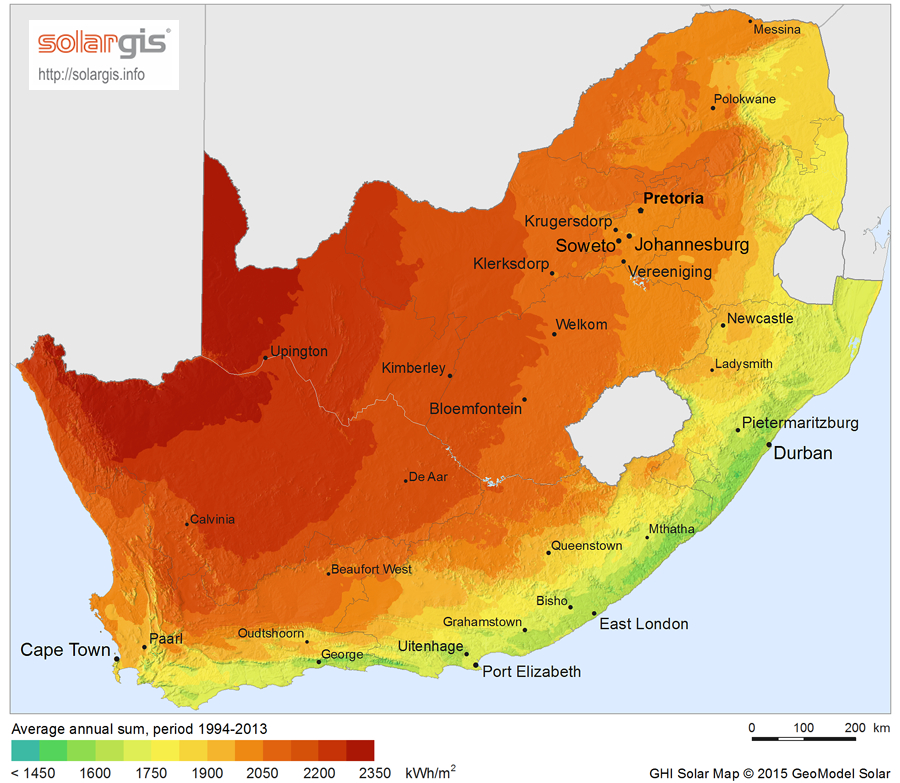
\includegraphics[width=0.95\textwidth]{FIG/SA_GHI}
                \caption{Global Horizontal Irradiation \cite{SolarGIS2015a}.}\label{fig:bild-links}
        \end{subfigure}%
        ~
        \begin{subfigure}[b]{0.5\textwidth}
                \centering
                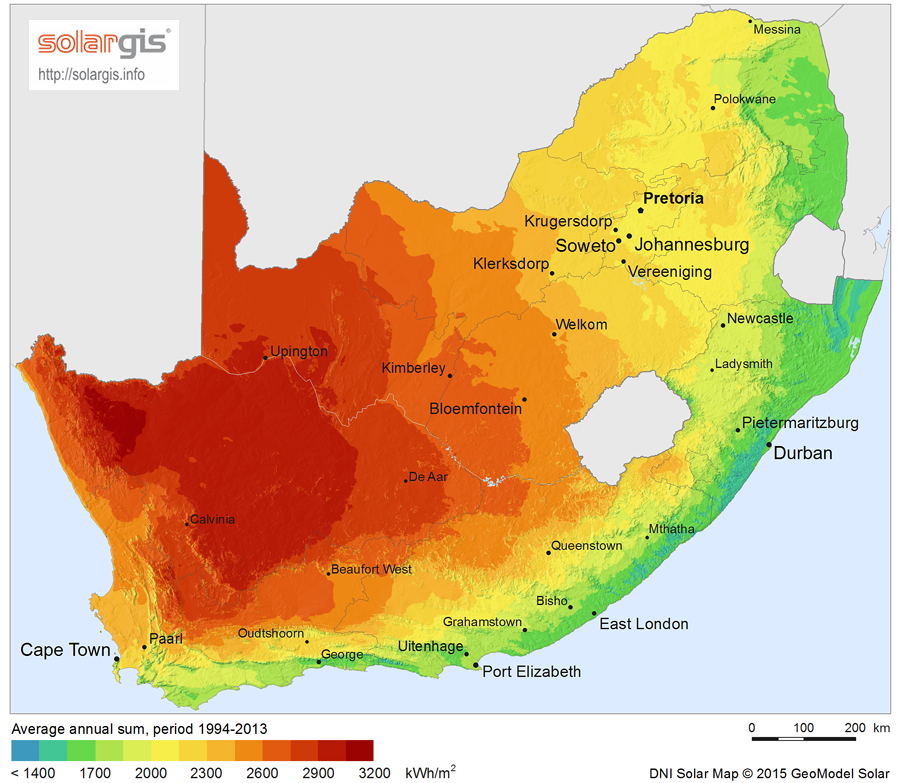
\includegraphics[width=0.95\textwidth]{FIG/SA_DNI}
                \caption{Direct Normal Irradiation \cite{SolarGIS2015b}.}\label{fig:bild-rechts}
        \end{subfigure}
        \caption{Solar radiation maps of South Africa.}\label{irradiation}
\end{figure}
\pagebreak
\section{Solar power plants in SA}
South Africa started there expansion in the field of solar power plants in the first round of the Renewable Energy Independent Power Producer Procurement Program (REIPPPP) in 2011. Now in 2015 starts the fourth round of the REIPPPP. Figure \ref{Solar-map} shows the allocation of all solar power plants of the REIPPPP. PV-power plants are marked in yellow and CSP-power plants are marked in orange. The numbers in the single marks expose in which REIPPPP-Round it belongs.
\begin{figure}[h!] % Solar-map
\centering
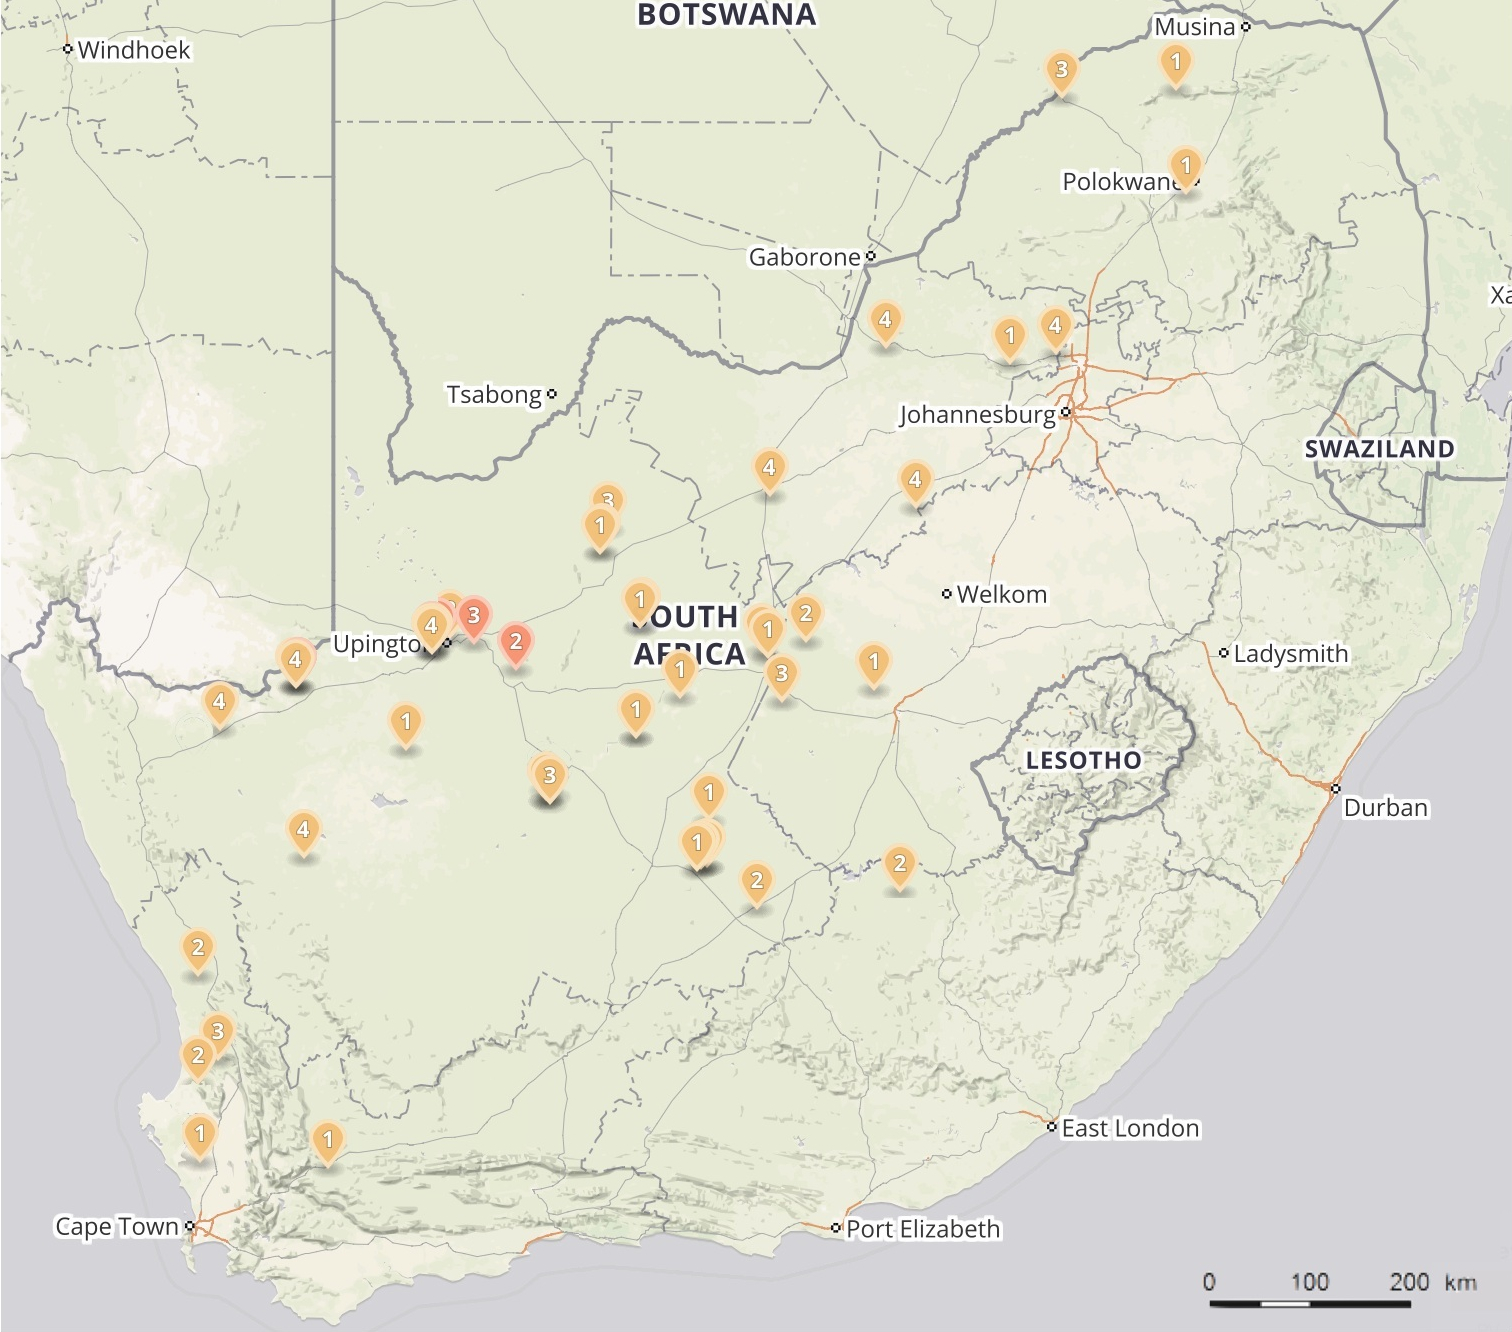
\includegraphics[width=1\linewidth]{FIG/Solar-map}
\caption[Allocation of all REIPPPP solar power plants in SA.]{Allocation of all REIPPPP solar power plants in SA \cite{Forder2015}.}\label{Solar-map}
\end{figure}

Currently SA has 26 fully operational PV-power plants with a total capacity of 1~048.7~MW, further seven PV-power plants with 135.35~MW are under construction, four more with 307.5~MW awaiting construction (approved \& financed) and there are six more PV-power plants in approvals, planning and financing with a total capacity of 415~MW. 

Mainly PV-power plants are allocated in the Northern Cape. So 26 of 39 of the operational and planed plants are located there. Five more in the Western Cape, three each in the provinces Free State and Limpopo and each one in Eastern Cape and the North-West Province. \cite{Forder2015}



"KaXu Solar One" is the first fully operational CSP-plant in SA and is shown in Figure \ref{KaXu-solar-field}. It is using parabolic trough technology and a 2.5~h thermal energy storage for generating of 100~MW capacity electricity. The CSP-plants "Khi Solar One" and "Bokpoort CSP Project" with a capacity of each 50~MW are under construction. Further three CSP-plants are awaiting construction, they have all a capacity of each 100~MW. 

All six CSP-plants are located in the region around the cites to Upington or Pofadder in the Northern Cape. This region is predestined for CSP-plants, because it has high DNI (around~2~900~kWh/m\textsuperscript{2}/a) and a water connection through the Orange River. \cite{Forder2015}
\begin{figure}[!h]
\centering
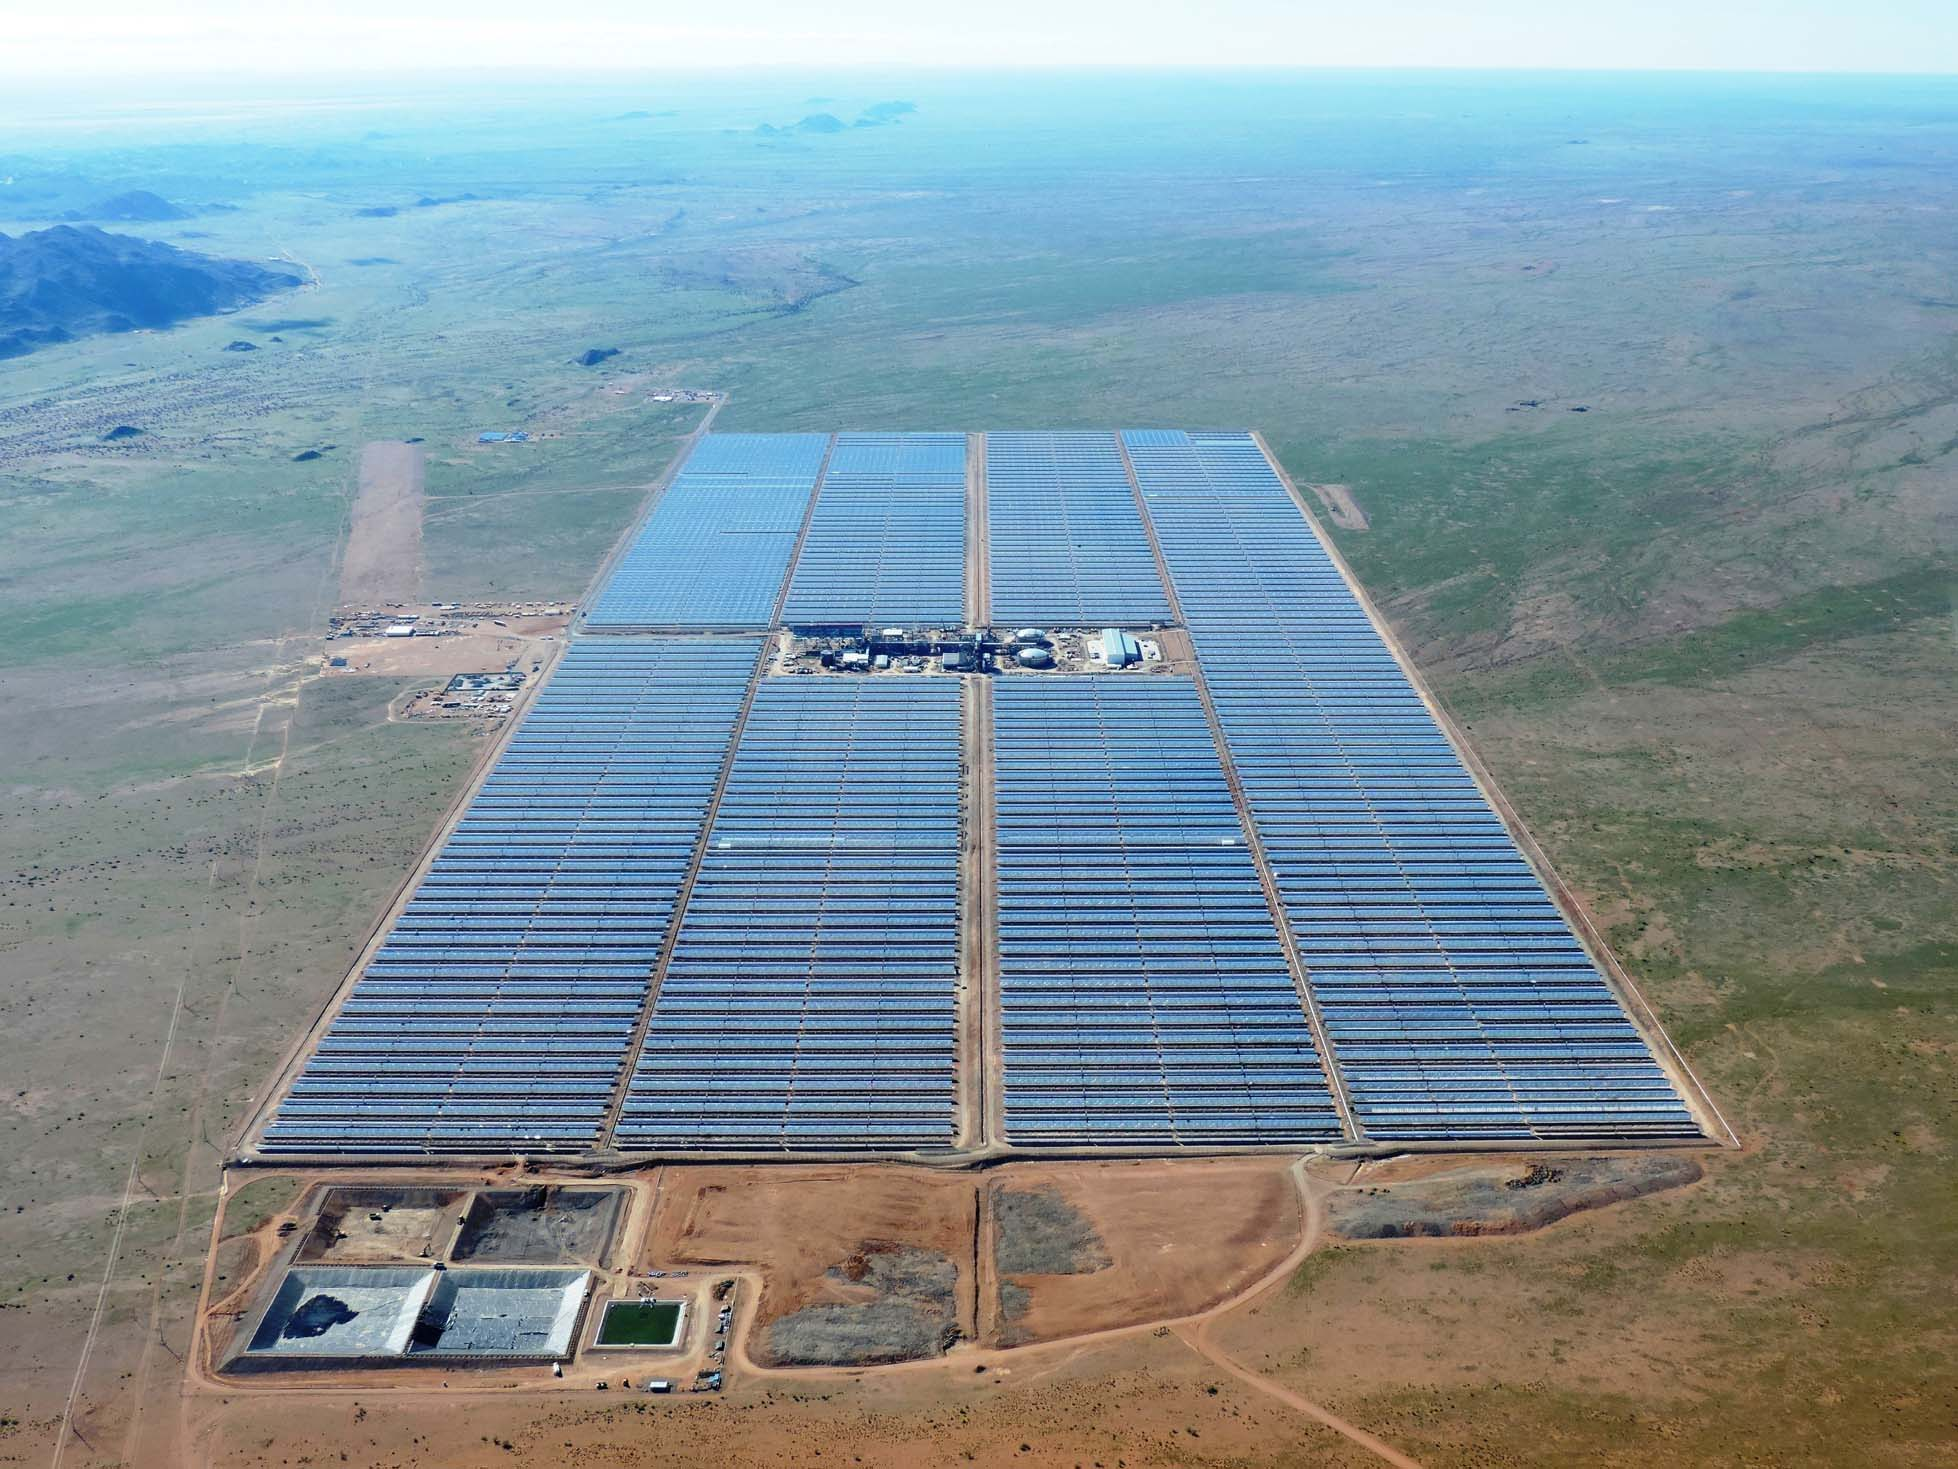
\includegraphics[width=1\linewidth]{FIG/KaXu-solar-field}
\caption[KaXu Solar One, a 100 MW parabolic trough plant with 2.5 hours of thermal storage in molten salts.]{KaXu Solar One, a 100 MW parabolic trough plant with 2.5 hours of thermal storage in molten salts \cite{AbengoaSolar2015}.}\label{KaXu-solar-field}
\end{figure}

\pagebreak
